\documentclass{article}
\usepackage{graphicx} % Required for inserting images
\usepackage{amsmath}
\usepackage{amsfonts}
\usepackage[margin=2.5cm]{geometry}

\title{CS229 - Problem Set 3}
\author{Or Haifler}
\date{November 2023}

\begin{document}

\maketitle

\section*{Exercise 1}
\subsection*{(a)}
\begin{align*}
    & \frac{\partial l}{\partial w_{1,2}^{[1]}}=\frac{\partial l}{\partial o}\cdot\frac{\partial o}{\partial h_{2}}\cdot\frac{\partial h_{2}}{\partial w_{1,2}^{[1]}}=\frac{2}{m}\sum_{i=1}^{m}(o^{(i)}-y^{(i)})\cdot o^{(i)}(1-o^{(i)})w_{2}^{[2]}\cdot h_{2}^{(i)}(1-h_{2}^{(i)})x_{1}^{(i)} \\
    & w_{1,2}^{[1]}:=w_{1,2}^{[1]}-\alpha\cdot\frac{2w_{2}^{[2]}}{m}\sum_{i=1}^{m}(o^{(i)}-y^{(i)})\cdot o^{(i)}(1-o^{(i)})\cdot h_{2}^{(i)}(1-h_{2}^{(i)})x_{1}^{(i)},h_{2}^{(i)}=^{x_{0}^{(i)}=1}\sigma\Big(\sum_{j=0}^{2}w_{j,2}^{[1]}x_{j}^{(i)}\Big)
\end{align*}

\subsection*{(b)}
Yes, we can use each hidden layer as a linear classifier, and choose each decision boundary to be one of the triangle sides

\subsection*{(c)}
No, if we'll use this setting, the model will be a composition of linear layers, which is a linear classifier, but the data set isn't linearly separable

\newpage

\section*{Exercise 2}
\subsection*{(a)}
\begin{align*}
    & D_{\text{KL}}(P\|Q)=\mathbb{E}_{z\sim P(Z)}[\log\frac{P(z)}{Q(z)}]=\sum_{x\in\mathcal{X}}P(z)\log\frac{P(z)}{Q(z)}=-\sum_{x\in\mathcal{X}}P(z)\log\frac{Q(z)}{P(z)}=\mathbb{E}_{z\sim P(Z)}[-\log\frac{Q(z)}{P(z)}]                      \\
    & \mathbb{E}_{z\sim P(Z)}[-\log\frac{Q(z)}{P(z)}]\ge^{Jensen}-\log\Big(\mathbb{E}_{z\sim P(Z)}[\frac{Q(z)}{P(z)}]\Big),\mathbb{E}_{z\sim P(Z)}[\frac{Q(z)}{P(z)}]=\sum_{x\in\mathcal{X}}P(z)\frac{Q(z)}{P(z)}=\sum_{x\in\mathcal{X}}Q(z)=1 \\
    & D_{\text{KL}}(P\|Q)=\mathbb{E}_{z\sim P(Z)}[-\log\frac{Q(z)}{P(z)}]\ge-\log(1)=0
\end{align*}

\subsection*{(b)}
\begin{align*}
    & D_{KL}(P(X,Y)\|Q(X,Y))=\mathbb{E}_{x,y\sim P(X,Y)}[\log\frac{P(x,y)}{Q(x,y)}]=\sum_{x\in\mathcal{X}}\sum_{y\in\mathcal{Y}}P(x,y)\log\frac{P(x,y)}{Q(x,y)}                                                                                                                                             \\
    & D_{KL}(P(X)\|Q(X))+D_{KL}(P(Y|X)\|Q(Y|X))=\mathbb{E}_{x\sim P(X)}[\log\frac{P(x)}{Q(x)}]+\mathbb{E}_{x\sim P(X)}[\mathbb{E}_{y\sim P(Y)}[\log\frac{P(y|x)}{Q(y|x)}]]                                                                                                                                  \\
    & =\sum_{x\in\mathcal{X}}P(x)\log\frac{P(x)}{Q(x)}+\sum_{x\in\mathcal{X}}P(x)\Big(\sum_{y\in\mathcal{Y}}P(y|X=x)\log\frac{P(y|X=x)}{Q(y|X=x)}\Big)                                                                                                                                                      \\
    & =\sum_{x\in\mathcal{X}}P(x)\Big(\sum_{y\in\mathcal{Y}}P(y|X=x)\log\frac{P(y|X=x)}{Q(y|X=x)}+\log\frac{P(x)}{Q(x)}\Big)                                                                                                                                                                                \\
    & =\sum_{x\in\mathcal{X}}P(x)\Big(\sum_{y\in\mathcal{Y}}\frac{P(y,x)}{P(x)}\log\frac{\frac{P(y,x)}{P(x)}}{\frac{Q(y,x)}{Q(x)}}+\log\frac{P(x)}{Q(x)}\Big)=\sum_{x\in\mathcal{X}}P(x)\Big(\sum_{y\in\mathcal{Y}}\frac{P(y,x)}{P(x)}\log\frac{P(y,x)}{Q(y,x)}\frac{Q(x)}{P(x)}+\log\frac{P(x)}{Q(x)}\Big) \\
    & =\sum_{x\in\mathcal{X}}P(x)\Big(\sum_{y\in\mathcal{Y}}\frac{P(y,x)}{P(x)}\log\frac{P(y,x)}{Q(y,x)}-\log\frac{P(x)}{Q(x)}+\log\frac{P(x)}{Q(x)}\Big)=\sum_{x\in\mathcal{X}}P(x)\Big(\sum_{y\in\mathcal{Y}}\frac{P(y,x)}{P(x)}\log\frac{P(y,x)}{Q(y,x)}\Big)                                            \\
    & =\sum_{x\in\mathcal{X}}\sum_{y\in\mathcal{Y}}P(x,y)\log\frac{P(x,y)}{Q(x,y)}=D_{KL}(P(X,Y)\|Q(X,Y))
\end{align*}

\subsection*{(c)}
\begin{align*}
    & \underset{\theta}{\arg\min}D_{KL}(\hat{P}\|P_{\theta})=\underset{\theta}{\arg\min}\sum_{x\in\mathcal{X}}\hat{P}(x)\log\frac{\hat{P}(x)}{P_{\theta}(x)}=\underset{\theta}{\arg\min}\sum_{x\in\mathcal{X}}\hat{P}(x)\log\hat{P}(x)-\underset{\theta}{\arg\min}\sum_{x\in\mathcal{X}}\hat{P}(x)\log P_{\theta}(x) \\
    & =-\underset{\theta}{\arg\min}\sum_{x\in\mathcal{X}}\hat{P}(x)\log P_{\theta}(x)=\underset{\theta}{\arg\max}\sum_{x\in\mathcal{X}}\hat{P}(x)\log P_{\theta}(x)                                                                                                                                                  \\
    & =^{\hat{P}(x)=0,x\not=x^{(i)}}\underset{\theta}{\arg\max}\sum_{i=1}^{m}\hat{P}(x^{(i)})\log P_{\theta}(x^{(i)})=\underset{\theta}{\arg\max}\sum_{i=1}^{m}\log P_{\theta}(x^{(i)})
\end{align*}

\newpage

\section*{Exercise 3}
\subsection*{(a)}
\begin{align*}
    & \mathbb{E}_{y\sim p(y;\theta)}[\nabla_{\theta^{'}}\log p(y;\theta^{'})|_{\theta^{'}=\theta}]=\int_{-\infty}^{\infty}p(y;\theta^{'})\nabla_{\theta^{'}}\log p(y;\theta^{'})dy=\int_{-\infty}^{\infty}p(y;\theta^{'})\frac{1}{p(y;\theta^{'})}\nabla_{\theta^{'}}p(y;\theta^{'})dy \\
    & =\int_{-\infty}^{\infty}\nabla_{\theta^{'}}p(y;\theta^{'})dy=\nabla_{\theta^{'}}\int_{-\infty}^{\infty}p(y;\theta^{'})dy=0
\end{align*}

\subsection*{(b)}
\begin{align*}
    & \mathcal{I}(\theta)=\mathbb{E}_{y\sim p(y;\theta)}[\Big(\nabla_{\theta^{'}}\log p(y;\theta^{'})-\mathbb{E}_{y\sim p(y;\theta)}[\nabla_{\theta^{'}}\log p(y;\theta^{'})]\Big)\Big(\nabla_{\theta^{'}}\log p(y;\theta^{'})-\mathbb{E}_{y\sim p(y;\theta)}[\nabla_{\theta^{'}}\log p(y;\theta^{'})]\Big)^{T}] \\
    & =^{(a)}\mathbb{E}_{y\sim p(y;\theta)}[\Big(\nabla_{\theta^{'}}\log p(y;\theta^{'})-0\Big)\Big(\nabla_{\theta^{'}}\log p(y;\theta^{'})-0\Big)^{T}]=\mathbb{E}_{y\sim p(y;\theta)}[\nabla_{\theta^{'}}\log p(y;\theta^{'})\nabla_{\theta^{'}}\log p(y;\theta^{'})^{T}]
\end{align*}

\subsection*{(c)}
\begin{align*}
    & \mathbb{E}_{y\sim p(y;\theta)}[\nabla_{\theta^{'}}\log p(y;\theta^{'})\nabla_{\theta^{'}}\log p(y;\theta^{'})^{T}]_{ij}=\mathbb{E}_{y\sim p(y;\theta)}[\frac{\partial\log p(y;\theta^{'})}{\partial\theta_{i}^{'}}\frac{\partial\log p(y;\theta^{'})}{\partial\theta_{j}^{'}}]                                                                                                                                                                 \\
    & =\mathbb{E}_{y\sim p(y;\theta)}[\frac{1}{p(y;\theta^{'})^{2}}\frac{\partial^{2}p(y;\theta^{'})}{\partial\theta_{j}^{'}\partial\theta_{i}^{'}}]=\mathbb{E}_{y\sim p(y;\theta)}[\frac{1}{p(y;\theta^{'})^{2}}\frac{\partial^{2}p(y;\theta^{'})}{\partial\theta_{j}^{'}\partial\theta_{i}^{'}}]                                                                                                                                                   \\
    & \mathbb{E}_{y\sim p(y;\theta)}[-\nabla_{\theta^{'}}^{2}\log p(y;\theta^{'})]_{ij}=\mathbb{E}_{y\sim p(y;\theta)}[\frac{1}{p(y;\theta^{'})^{2}}\frac{\partial^{2}p(y;\theta^{'})}{\partial\theta_{j}^{'}\partial\theta_{i}^{'}}-\frac{1}{p(y;\theta)}\frac{\partial^{2}p(y;\theta^{'})}{\partial\theta_{j}^{'}\partial\theta_{i}^{'}}]                                                                                                          \\
    & =\mathbb{E}_{y\sim p(y;\theta)}[\frac{1}{p(y;\theta^{'})^{2}}\frac{\partial^{2}p(y;\theta^{'})}{\partial\theta_{j}^{'}\partial\theta_{i}^{'}}]-\mathbb{E}_{y\sim p(y;\theta)}[\frac{1}{p(y;\theta^{'})}\frac{\partial^{2}p(y;\theta^{'})}{\partial\theta_{j}^{'}\partial\theta_{i}^{'}}]                                                                                                                                                       \\
    & =\mathbb{E}_{y\sim p(y;\theta)}[\frac{1}{p(y;\theta^{'})^{2}}\frac{\partial^{2}p(y;\theta^{'})}{\partial\theta_{j}^{'}\partial\theta_{i}^{'}}]-\int_{-\infty}^{\infty}p(y;\theta^{'})\frac{1}{p(y;\theta^{'})}\frac{\partial^{2}p(y;\theta^{'})}{\partial\theta_{j}^{'}\partial\theta_{i}^{'}}dy                                                                                                                                               \\
    & =\mathbb{E}_{y\sim p(y;\theta)}[\frac{1}{p(y;\theta^{'})^{2}}\frac{\partial^{2}p(y;\theta^{'})}{\partial\theta_{j}^{'}\partial\theta_{i}^{'}}]-\frac{\partial^{2}p(y;\theta^{'})}{\partial\theta_{j}^{'}\partial\theta_{i}^{'}}\int_{-\infty}^{\infty}p(y;\theta^{'})dy=\mathbb{E}_{y\sim p(y;\theta)}[\frac{1}{p(y;\theta^{'})^{2}}\frac{\partial^{2}p(y;\theta^{'})}{\partial\theta_{j}^{'}\partial\theta_{i}^{'}}]=\mathcal{I}(\theta)_{ij}
\end{align*}

\subsection*{(d)}
\begin{align*}
    & f(\tilde{\theta})=D_{KL}(p_{\theta}\|p_{\tilde{\theta}})\approx\underbrace{D_{KL}(p_{\theta}\|p_{\theta})}_{0}+(\tilde{\theta}-\theta)^{T}\nabla_{\theta^{'}}f(\theta^{'})|_{\theta^{'}=\theta}+\frac{1}{2}(\tilde{\theta}-\theta)^{T}(\nabla_{\theta^{'}}^{2}f(\theta^{'})|_{\theta^{'}=\theta}(\tilde{\theta}-\theta)                                                                                                                                                                                                  \\
    & =d^{T}\nabla_{\theta^{'}}D_{KL}(p_{\theta}\|p_{\tilde{\theta}})+\frac{1}{2}d^{T}(\nabla_{\theta^{'}}^{2}D_{KL}(p_{\theta}\|p_{\tilde{\theta}}))d=d^{T}\nabla_{\theta^{'}}\mathbb{E}_{y\sim p(y;\theta^{'})}[\log\frac{p_{\theta}(y;\theta^{'})}{p_{\tilde{\theta}}(y;\theta^{'})}]+\frac{1}{2}d^{T}\nabla_{\theta^{'}}^{2}\mathbb{E}_{y\sim p(y;\theta^{'})}[\log\frac{p_{\theta}(y;\theta^{'})}{p_{\tilde{\theta}}(y;\theta^{'})}]d                                                                                     \\
    & =^{(a)+(c)}\underbrace{d^{T}\mathbb{E}_{y\sim p(y;\theta^{'})}[\nabla_{\theta^{'}}\log\frac{p_{\theta}(y)}{p_{\tilde{\theta}}(y)}]}_{d^{T}0}+\underbrace{\frac{1}{2}d^{T}\nabla_{\theta^{'}}^{2}\mathbb{E}_{y\sim p(y;\theta^{'})}[\log p_{\theta}(y;\theta^{'})]d}_{\frac{1}{2}d^{T}0d}+\text{\ensuremath{\underbrace{\frac{1}{2}d^{T}\mathbb{E}_{y\sim p(y;\theta^{'})}[-\nabla_{\theta^{'}}^{2}\log p_{\tilde{\theta}}(y;\theta^{'})]d}_{\frac{1}{2}d^{T}\mathcal{I}(\theta)d}=\frac{1}{2}d^{T}\mathcal{I}(\theta)d}}
\end{align*}

\subsection*{(e)}
\begin{align*}
    & \mathcal{L}(d,\lambda)=\ell(\theta+d)-\lambda\Big(D_{KL}(p_{\theta}\|p_{\tilde{\theta}})-c\Big)\approx\log p(y;\theta)+d^{T}\frac{\nabla_{\theta^{'}}p(y;\theta')|_{\theta'=\theta}}{p(y;\theta)}-\lambda\Big(\frac{1}{2}d^{T}\mathcal{I}(\theta)d-c\Big)                                                                                            \\
    & \nabla_{d}\mathcal{L}(d,\lambda)\approx\frac{\nabla_{\theta^{'}}p(y;\theta')|_{\theta'=\theta}}{p(y;\theta)}-\lambda\mathcal{I}(\theta)d=0\implies d=\frac{1}{\lambda}\mathcal{I}(\theta)^{-1}\frac{\nabla_{\theta^{'}}p(y;\theta')|_{\theta'=\theta}}{p(y;\theta)}                                                                                  \\
    & \nabla_{\lambda}\mathcal{L}(d,\lambda)\approx c-\frac{1}{2}d^{T}\mathcal{I}(\theta)d=c-\frac{1}{\lambda}\mathcal{I}(\theta)^{-1}\Big[\frac{\nabla_{\theta^{'}}p(y;\theta')|_{\theta'=\theta}}{p(y;\theta)}\Big]^{T}\mathcal{I}(\theta)\frac{1}{\lambda}\mathcal{I}(\theta)^{-1}\frac{\nabla_{\theta^{'}}p(y;\theta')|_{\theta'=\theta}}{p(y;\theta)} \\
    & =c-\frac{1}{2\lambda^{2}p(y;\theta)^{2}}\nabla_{\theta^{'}}p(y;\theta')|_{\theta'=\theta}^{T}\mathcal{I}(\theta)^{-1}\nabla_{\theta^{'}}p(y;\theta')|_{\theta'=\theta}                                                                                                                                                                               \\
    & \nabla_{\lambda}\mathcal{L}(d,\lambda)=0\implies\lambda=\sqrt{\frac{1}{2cp(y;\theta)^{2}}\nabla_{\theta^{'}}p(y;\theta')|_{\theta'=\theta}^{T}\mathcal{I}(\theta)^{-1}\nabla_{\theta^{'}}p(y;\theta')|_{\theta'=\theta}}                                                                                                                             \\
    & d^{*}=\sqrt{\frac{2cp(y;\theta)^{2}}{\nabla_{\theta^{'}}p(y;\theta')|_{\theta'=\theta}^{T}\mathcal{I}(\theta)^{-1}\nabla_{\theta^{'}}p(y;\theta')|_{\theta'=\theta}}}\mathcal{I}(\theta)^{-1}\frac{\nabla_{\theta^{'}}p(y;\theta')|_{\theta'=\theta}}{p(y;\theta)}                                                                                   \\
    & =\sqrt{\frac{2c}{\nabla_{\theta^{'}}p(y;\theta')|_{\theta'=\theta}^{T}\mathcal{I}(\theta)^{-1}\nabla_{\theta^{'}}p(y;\theta')|_{\theta'=\theta}}}\mathcal{I}(\theta)^{-1}\nabla_{\theta^{'}}p(y;\theta')|_{\theta'=\theta}
\end{align*}

\subsection*{(f)}
In Newton's method, the update is $\theta := \theta - H^{-1}\nabla_{\theta}\ell(\theta)$, where the update using Natural gradient is $$\mathcal{I}(\theta)=\mathbb{E}_{y\sim p(y;\theta^{'})}[-\nabla_{\theta^{'}}^{2}\log p_{\tilde{\theta}}(y;\theta^{'})]=-\mathbb{E}_{y\sim p(y;\theta)}[H],\theta:=\theta+\tilde{d}=\theta-\frac{1}{\lambda}\mathbb{E}_{y\sim p(y;\theta)}[H]^{-1}\nabla_{\theta}\ell(\theta)$$

\newpage

\section*{Exercise 4}
\subsection*{(a)}
\begin{align*}
    & \ell_{\text{semi-sup}}(\theta^{(t+1)})=\ell_{\text{sup}}(\theta^{(t+1)})+\alpha\ell_{\text{unsup}}(\theta^{(t+1)})=\sum_{i=1}^{m}\log\sum_{z^{(i)}}p(x^{(i)},z^{(i)},\theta^{(t+1)})+\alpha\sum_{i=1}^{\tilde{m}}\log p(\tilde{x}^{(i)},z^{(i)},\theta^{(t+1)}) \\
    & \ge\sum_{i=1}^{m}\Big(\sum_{z^{(i)}}Q_{i}^{(t)}(z^{(i)})\log\frac{p(x^{(i)},z^{(i)},\theta^{(t+1)})}{Q_{i}^{(t)}(z^{(i)})}\Big)+\alpha\sum_{i=1}^{\tilde{m}}\log p(\tilde{x}^{(i)},z^{(i)},\theta^{(t+1)})                                                      \\
    & \ge\sum_{i=1}^{m}\Big(\sum_{z^{(i)}}Q_{i}^{(t)}(z^{(i)})\log\frac{p(x^{(i)},z^{(i)},\theta^{(t+1)})}{Q_{i}^{(t)}(z^{(i)})}\Big)+\alpha\sum_{i=1}^{\tilde{m}}\log p(\tilde{x}^{(i)},z^{(i)},\theta^{(t+1)})=\ell_{\text{semi-sup}}(\theta^{(t)})
\end{align*}

\subsection*{(b)}
\subsubsection*{E-step}
\begin{align*}
    & p(x^{(i)}|z^{(i)};\theta^{(t)})\sim\mathcal{N}(\Sigma_{i},\mu_{i}),p(z^{(i)}=j)=\phi_{j}                                                                                                                                                                                                               \\
    & w_{j}^{(i)}:=p(z^{(i)}=j|x^{(i)};\theta^{(t)})=\frac{p(x^{(i)}|z^{(i)}=j;\mu,\Sigma)p(z^{(i)}=j;\phi)}{\sum_{k}p(x^{(i)}|z^{(i)}=k;\mu,\Sigma)p(z^{(i)}=k;\phi)}                                                                                                                                       \\
    & =\frac{\frac{1}{(2\pi)^{n/2}(\det\Sigma_{j})^{1/2}}\exp\Big(-\frac{1}{2}(x^{(i)}-\mu_{j})^{T}\Sigma_{j}^{-1}(x^{(i)}-\mu_{j})^{T}\Big)\phi_{j}}{\sum_{k=1}^{j}\frac{1}{(2\pi)^{n/2}(\det\Sigma_{k})^{1/2}}\exp\Big(-\frac{1}{2}(x^{(i)}-\mu_{k})^{T}\Sigma_{k}^{-1}(x^{(i)}-\mu_{k})^{T}\Big)\phi_{k}}
\end{align*}
\subsubsection*{M-step}
I didn't have time to show the full derivation, but with Lagrange Multipliers one can see that $$\phi_{j}=\frac{\sum_{i=1}^{m}w_{j}^{(i)}+\alpha\sum_{i=1}^{\tilde{m}}\mathbb{I}{\tilde{z}^{(i)}=j}}{m+\alpha\tilde{m}}$$

Now, for the painful derivation
\begin{align*}
    & \nabla_{\mu_{j}}\ell_{\text{sup}}(\theta)=\sum_{i=1}^{\tilde{m}}\mathbb{I}{\tilde{z}^{(i)}=j}\Sigma_{j}^{-1}(\tilde{x}^{(i)}-\mu_{j}),\nabla_{\mu_{j}}\ell_{\text{unsup}}(\theta)=\sum_{i=1}^{m}w_{j}^{(i)}\Sigma_{j}^{-1}(x^{(i)}-\mu_{j})                                                                                                                                       \\
    & \nabla_{\mu_{j}}\ell_{\text{semi-sup}}(\theta)=\sum_{i=1}^{m}w_{j}^{(i)}\Sigma_{j}^{-1}(x^{(i)}-\mu_{j})+\alpha\sum_{i=1}^{\tilde{m}}\mathbb{I}{\tilde{z}^{(i)}=j}\Sigma_{j}^{-1}(\tilde{x}^{(i)}-\mu_{j})                                                                                                                                                                        \\
    & =\Sigma_{j}^{-1}\Big(\sum_{i=1}^{m}w_{j}^{(i)}x^{(i)}-\mu_{j}\sum_{i=1}^{m}w_{j}^{(i)}\Big)+\alpha\Sigma_{j}^{-1}\Big(\sum_{i=1}^{m}\mathbb{I}{\tilde{z}^{(i)}=j}x^{(i)}-\mu_{j}\sum_{i=1}^{m}\mathbb{I}{\tilde{z}^{(i)}=j}\Big)                                                                                                                                                  \\
    & =\Sigma_{j}^{-1}\Big[\sum_{i=1}^{m}w_{j}^{(i)}x^{(i)}-\mu_{j}\sum_{i=1}^{m}w_{j}^{(i)}-\alpha\Big(\sum_{i=1}^{m}\mathbb{I}{\tilde{z}^{(i)}=j}x^{(i)}-\mu_{j}\sum_{i=1}^{m}\mathbb{I}{\tilde{z}^{(i)}=j}\Big)\Big]                                                                                                                                                                 \\
    & =\Sigma_{j}^{-1}\Big[\sum_{i=1}^{m}w_{j}^{(i)}x^{(i)}+\alpha\sum_{i=1}^{m}\mathbb{I}{\tilde{z}^{(i)}=j}x^{(i)}-\mu_{j}\Big(\sum_{i=1}^{m}w_{j}^{(i)}+\alpha\sum_{i=1}^{\tilde{m}}\mathbb{I}{\tilde{z}^{(i)}=j}\Big)\Big]                                                                                                                                                          \\
    & \nabla_{\mu_{j}}\ell_{\text{semi-sup}}(\theta)=0\implies\mu_{j}=\frac{\sum_{i=1}^{m}w_{j}^{(i)}x^{(i)}+\alpha\sum_{i=1}^{\tilde{m}}\mathbb{I}{\tilde{z}^{(i)}=j}\tilde{x}^{(i)}}{\sum_{i=1}^{m}w_{j}^{(i)}+\alpha\sum_{i=1}^{\tilde{m}}\mathbb{I}{\tilde{z}^{(i)}=j}}                                                                                                             \\
    & \nabla_{\Sigma_{j}}\ell_{\text{sup}}(\theta)=\frac{1}{2}\Sigma_{j}^{-1}\Big(\sum_{i=1}^{\tilde{m}}\mathbb{I}{\tilde{z}^{(i)}=j}(\tilde{x}^{(i)}-\mu_{j})(\tilde{x}^{(i)}-\mu_{j})^{T}\Big)\Sigma_{j}^{-1}-\frac{1}{2}\sum_{i=1}^{\tilde{m}}\mathbb{I}{\tilde{z}^{(i)}=j}\Sigma_{j}^{-1}                                                                                           \\
    & \nabla_{\Sigma_{j}}\ell_{\text{unsup}}(\theta)=\frac{1}{2}\Sigma_{j}^{-1}\Big(\sum_{i=1}^{\tilde{m}}w_{j}^{(i)}(\tilde{x}^{(i)}-\mu_{j})(\tilde{x}^{(i)}-\mu_{j})^{T}\Big)\Sigma_{j}^{-1}-\frac{1}{2}\sum_{i=1}^{\tilde{m}}w_{j}^{(i)}\Sigma_{j}^{-1}                                                                                                                             \\
    & \nabla_{\Sigma_{j}}\ell_{\text{semi-sup}}(\theta)=\frac{1}{2}\Sigma_{j}^{-1}\Big(\sum_{i=1}^{\tilde{m}}w_{j}^{(i)}(\tilde{x}^{(i)}-\mu_{j})(\tilde{x}^{(i)}-\mu_{j})^{T}\Big)\Sigma_{j}^{-1}-\frac{1}{2}\sum_{i=1}^{\tilde{m}}w_{j}^{(i)}\Sigma_{j}^{-1}                                                                                                                          \\
    & +\frac{\alpha}{2}\Sigma_{j}^{-1}\Big(\sum_{i=1}^{\tilde{m}}\mathbb{I}{\tilde{z}^{(i)}=j}(\tilde{x}^{(i)}-\mu_{j})(\tilde{x}^{(i)}-\mu_{j})^{T}\Big)\Sigma_{j}^{-1}-\frac{\alpha}{2}\sum_{i=1}^{\tilde{m}}\mathbb{I}{\tilde{z}^{(i)}=j}\Sigma_{j}^{-1}                                                                                                                             \\
    & =\frac{1}{2}\Sigma_{j}^{-1}\Big(\sum_{i=1}^{\tilde{m}}w_{j}^{(i)}(\tilde{x}^{(i)}-\mu_{j})(\tilde{x}^{(i)}-\mu_{j})^{T}+\alpha\sum_{i=1}^{\tilde{m}}\mathbb{I}{\tilde{z}^{(i)}=j}(\tilde{x}^{(i)}-\mu_{j})(\tilde{x}^{(i)}-\mu_{j})^{T}\Big)\Sigma_{j}^{-1}                                                                                                                       \\
    & -\frac{1}{2}\Sigma_{j}^{-1}\Big(\sum_{i=1}^{\tilde{m}}w_{j}^{(i)}+\alpha\sum_{i=1}^{\tilde{m}}\mathbb{I}{\tilde{z}^{(i)}=j}\Big)                                                                                                                                                                                                                                                  \\
    & \nabla_{\Sigma_{j}}\ell_{\text{semi-sup}}(\theta)=0\implies\Sigma_{j}=\frac{\sum_{i=1}^{\tilde{m}}w_{j}^{(i)}(\tilde{x}^{(i)}-\mu_{j})(\tilde{x}^{(i)}-\mu_{j})^{T}+\alpha\sum_{i=1}^{\tilde{m}}\mathbb{I}{\tilde{z}^{(i)}=j}(\tilde{x}^{(i)}-\mu_{j})(\tilde{x}^{(i)}-\mu_{j})^{T}}{\sum_{i=1}^{\tilde{m}}w_{j}^{(i)}+\alpha\sum_{i=1}^{\tilde{m}}\mathbb{I}{\tilde{z}^{(i)}=j}}
\end{align*}

\newpage

\subsection*{(d),(e)}
\begin{figure}[h]
  \centering
  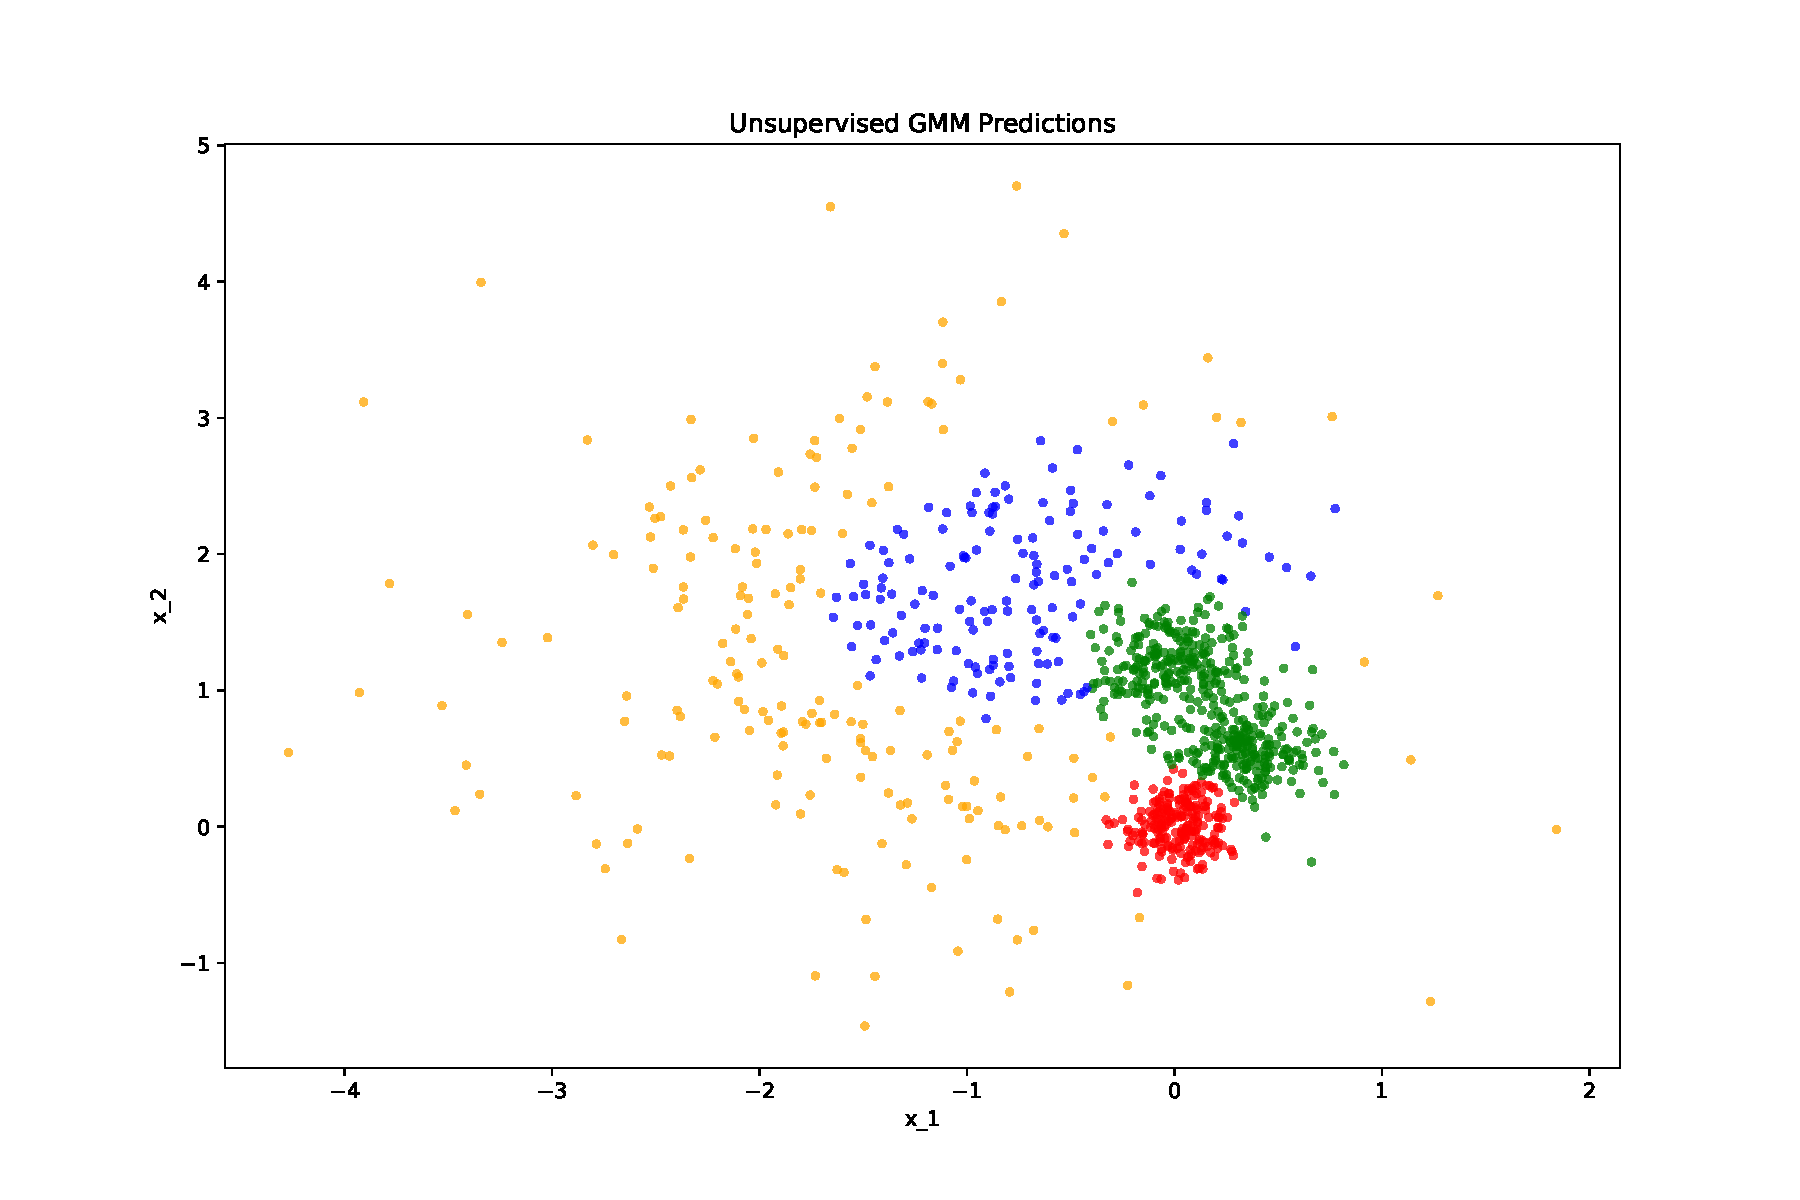
\includegraphics[width=1\textwidth]{images/p03_pred_0.pdf}
  \caption{Unsupervised GMM}
  \label{fig:enter-label}
\end{figure}

\begin{figure}
  \centering
  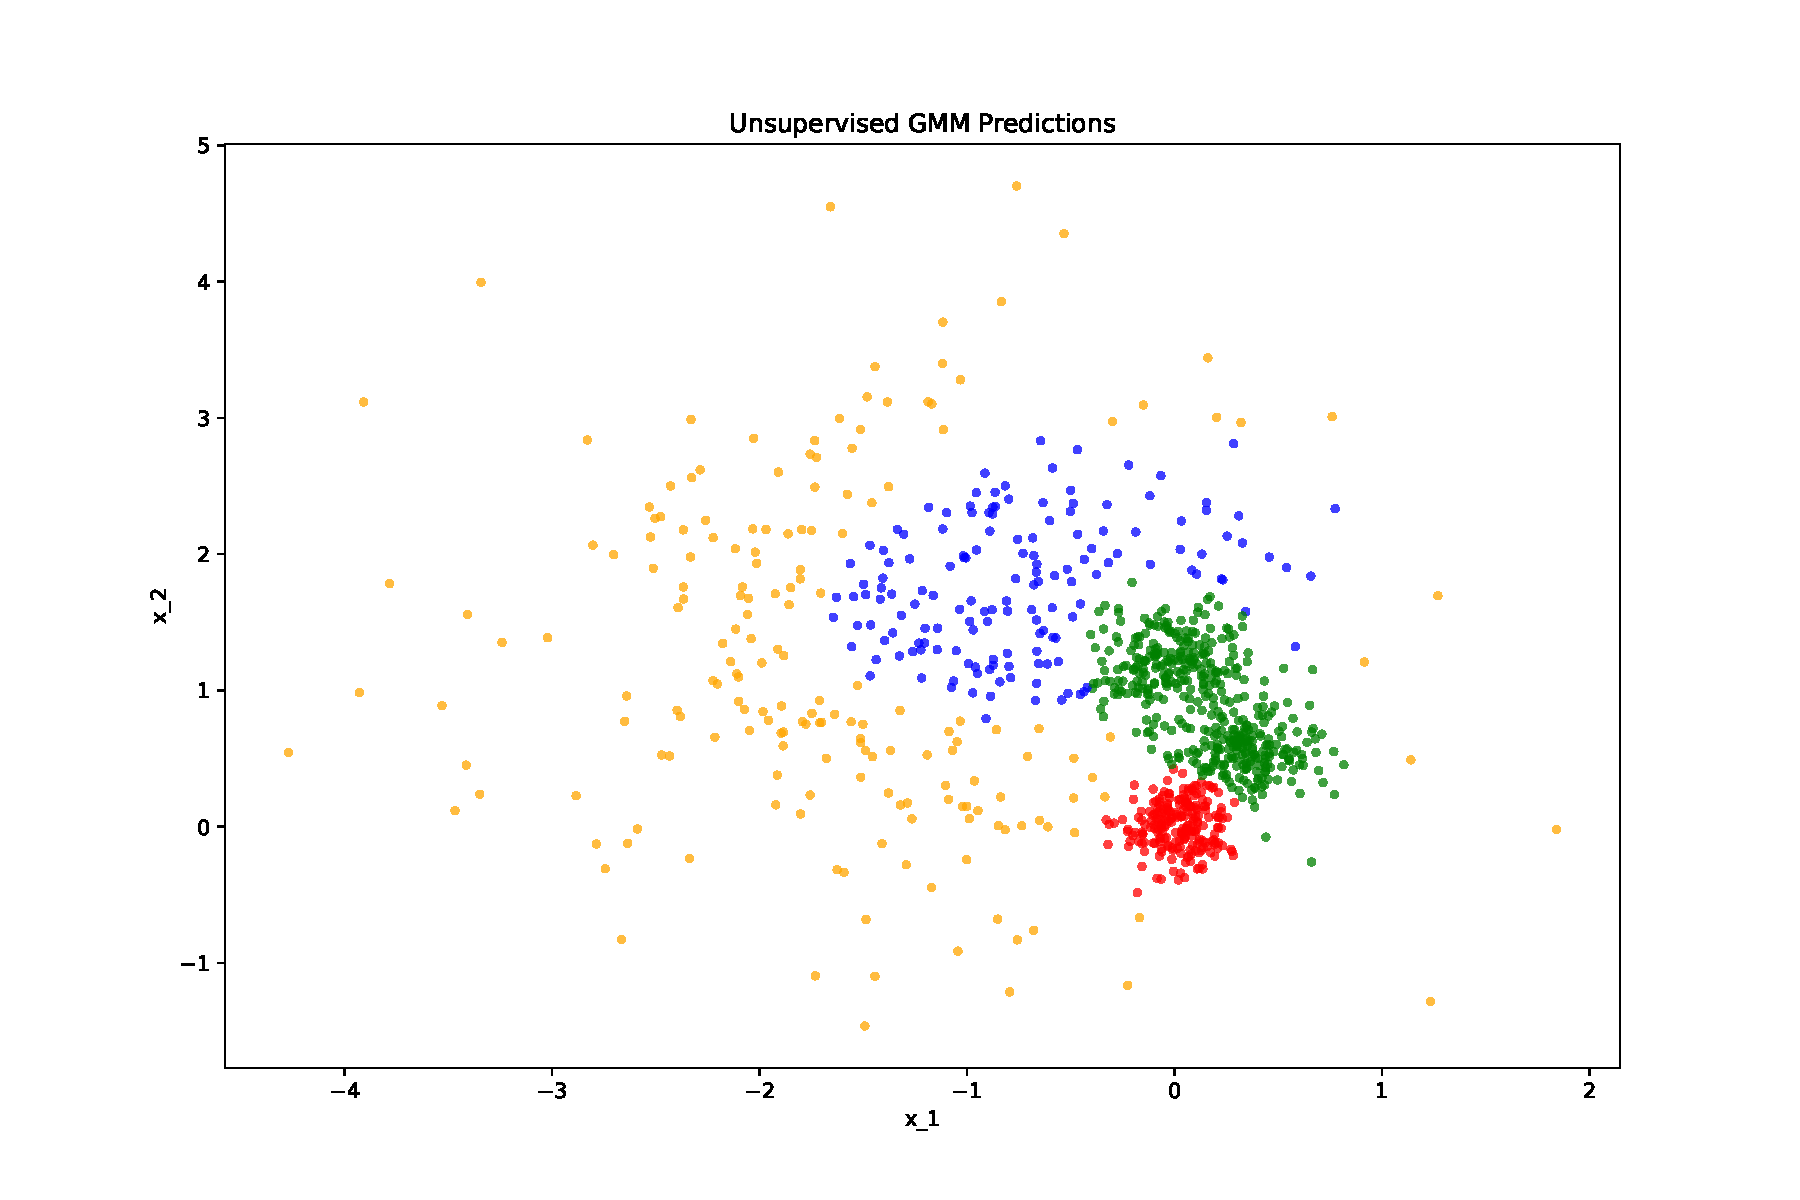
\includegraphics[width=1\textwidth]{images/p03_pred_1.pdf}
  \caption{Unsupervised GMM}
  \label{fig:enter-label}
\end{figure}

\begin{figure}
  \centering
  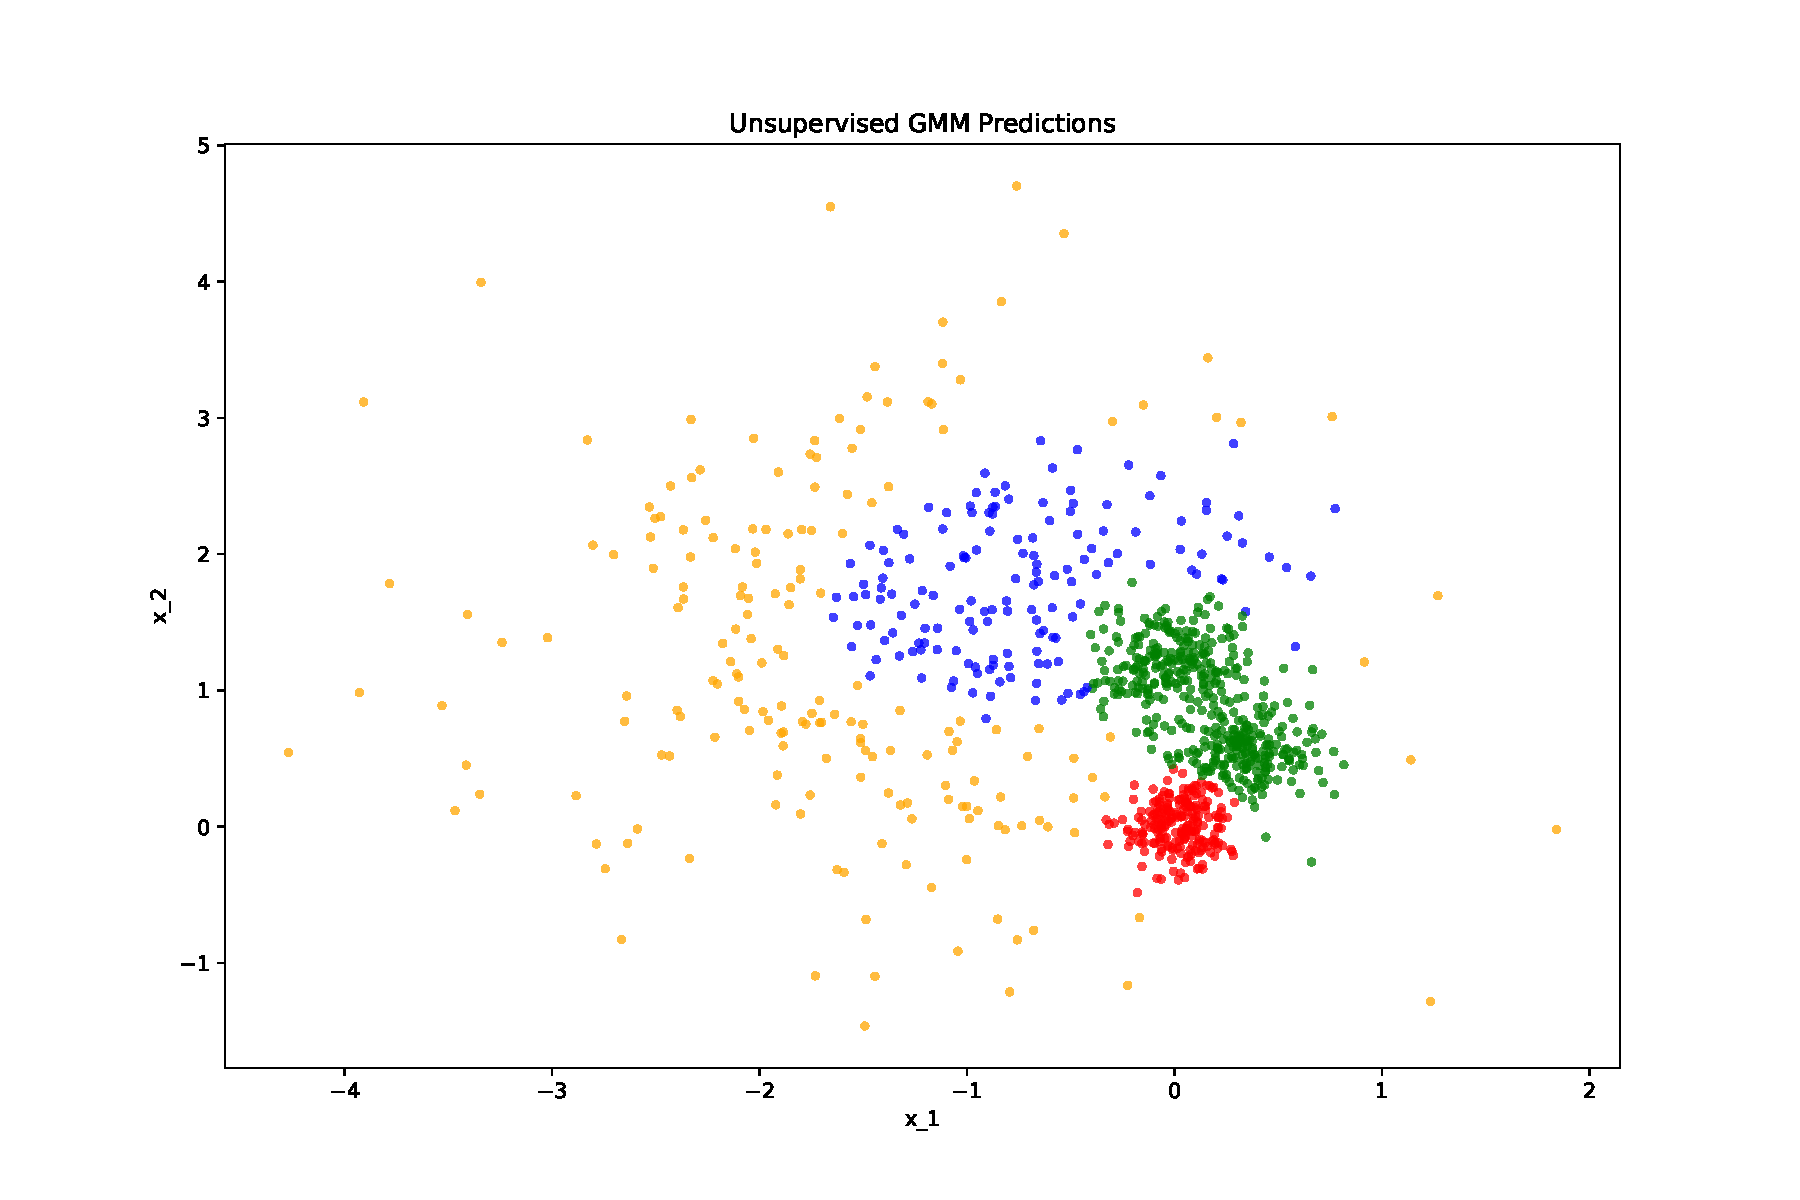
\includegraphics[width=1\textwidth]{images/p03_pred_2.pdf}
  \caption{Unsupervised GMM}
  \label{fig:enter-label}
\end{figure}

\begin{figure}
  \centering
  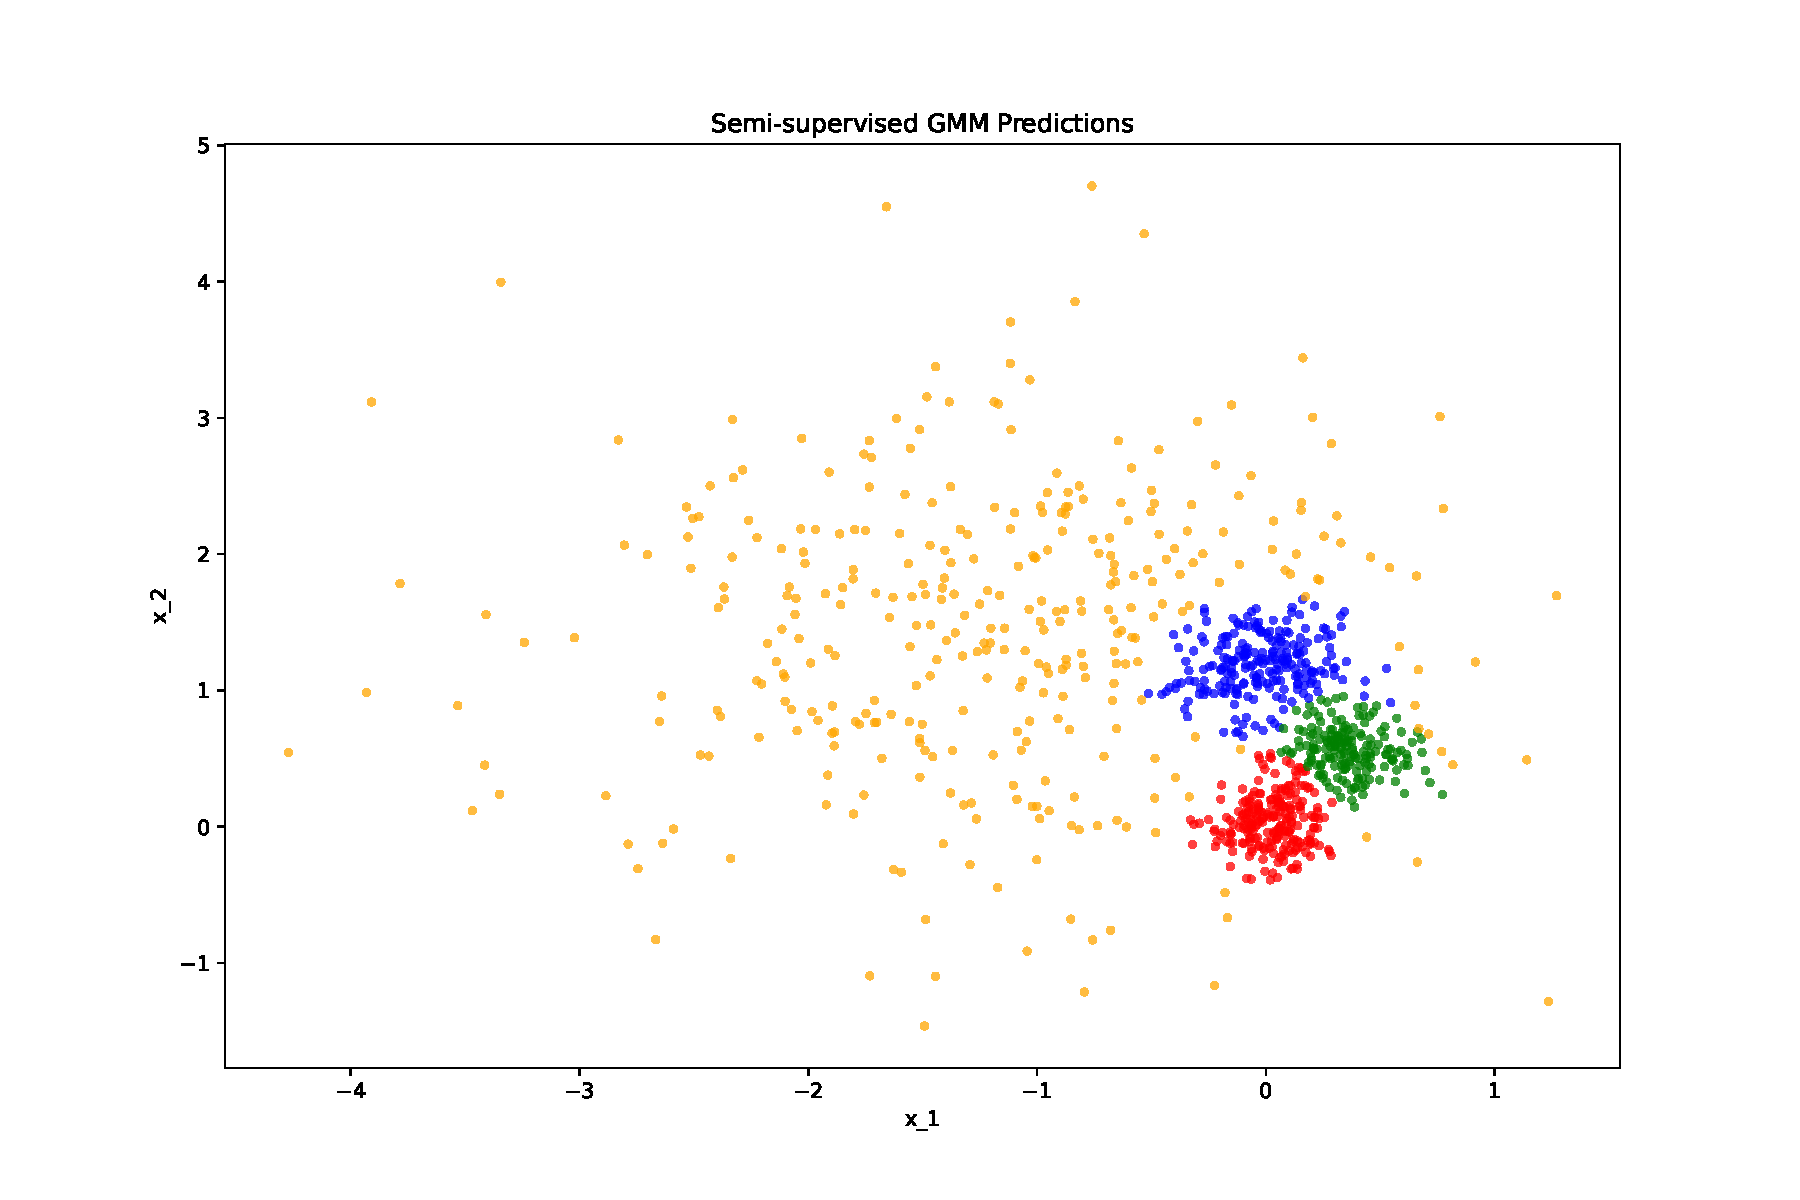
\includegraphics[width=1\textwidth]{images/p03_pred_ss_0.pdf}
  \caption{Semi-supervised GMM}
  \label{fig:enter-label}
\end{figure}

\begin{figure}
  \centering
  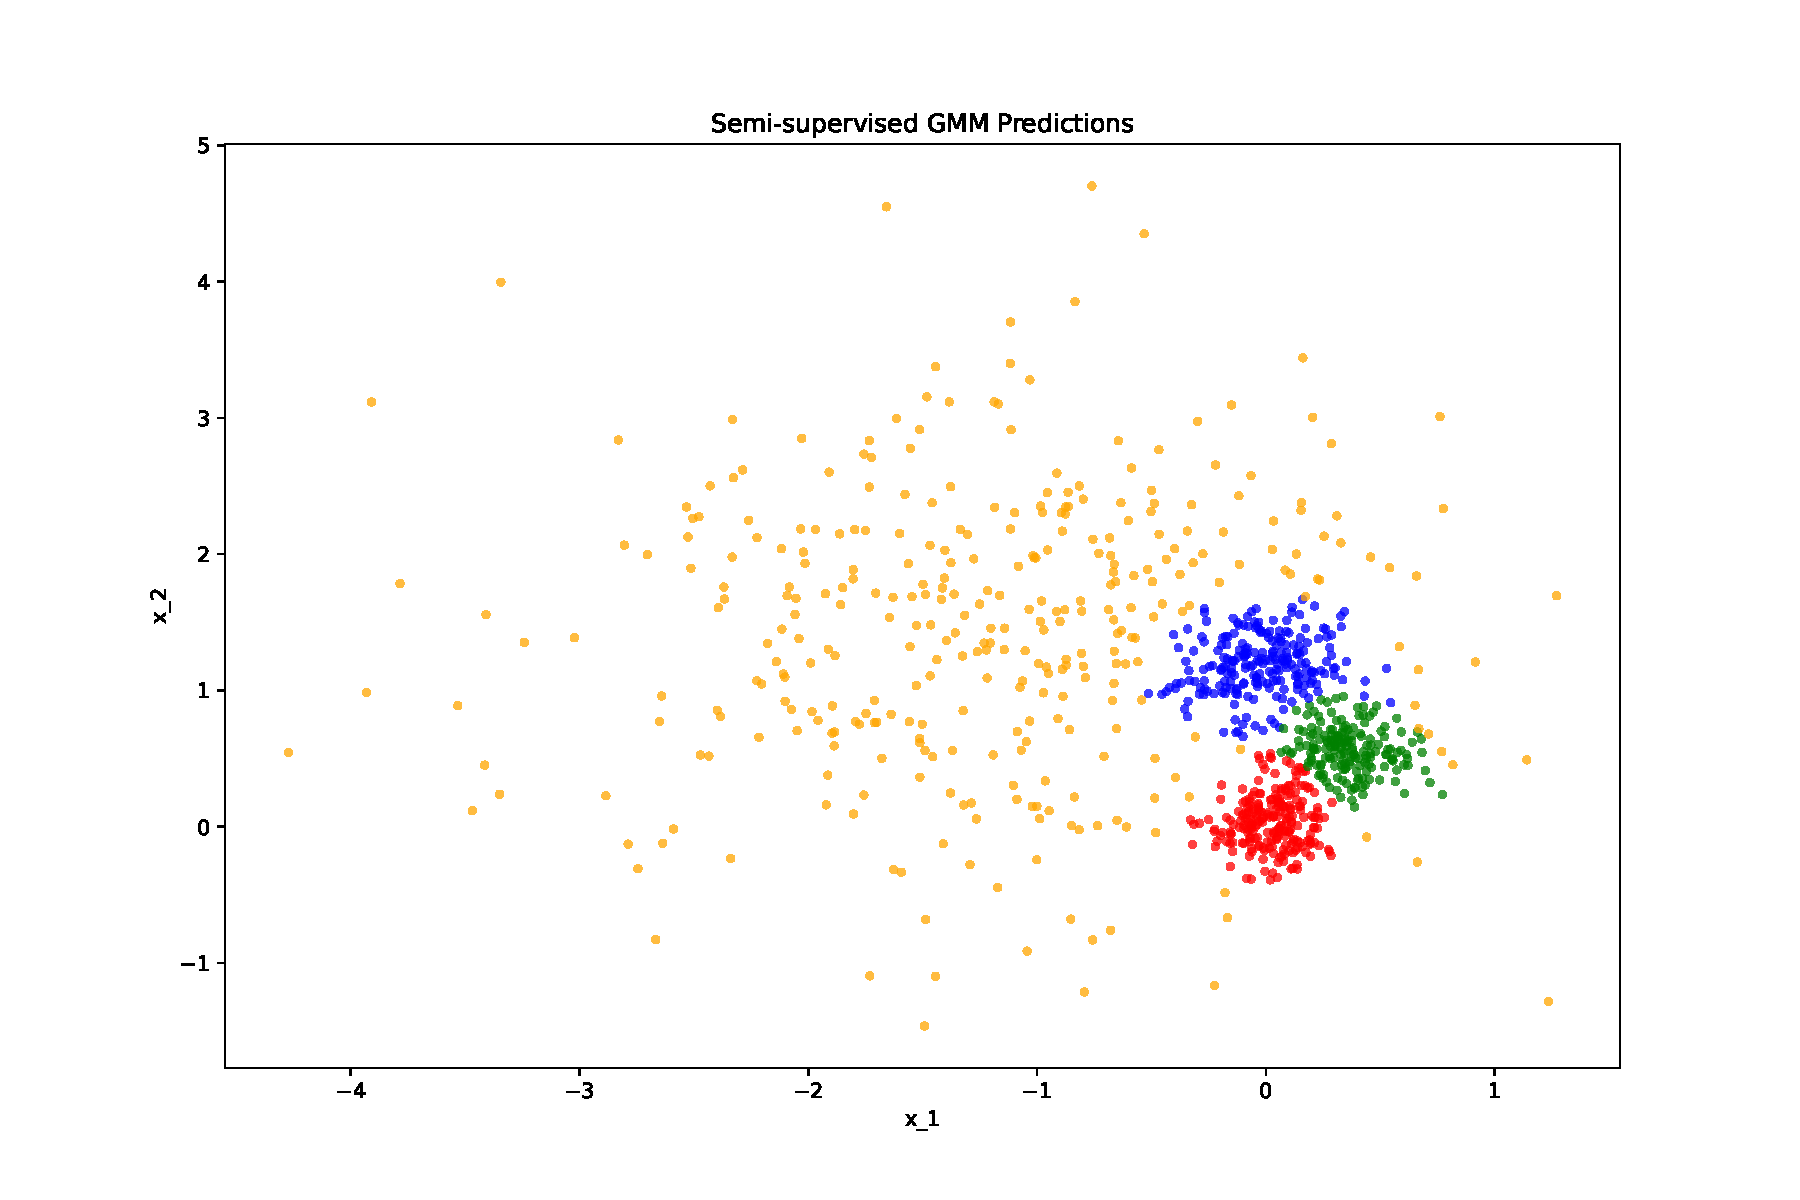
\includegraphics[width=1\textwidth]{images/p03_pred_ss_1.pdf}
  \caption{Semi-supervised GMM}
  \label{fig:enter-label}
\end{figure}

\begin{figure}
  \centering
  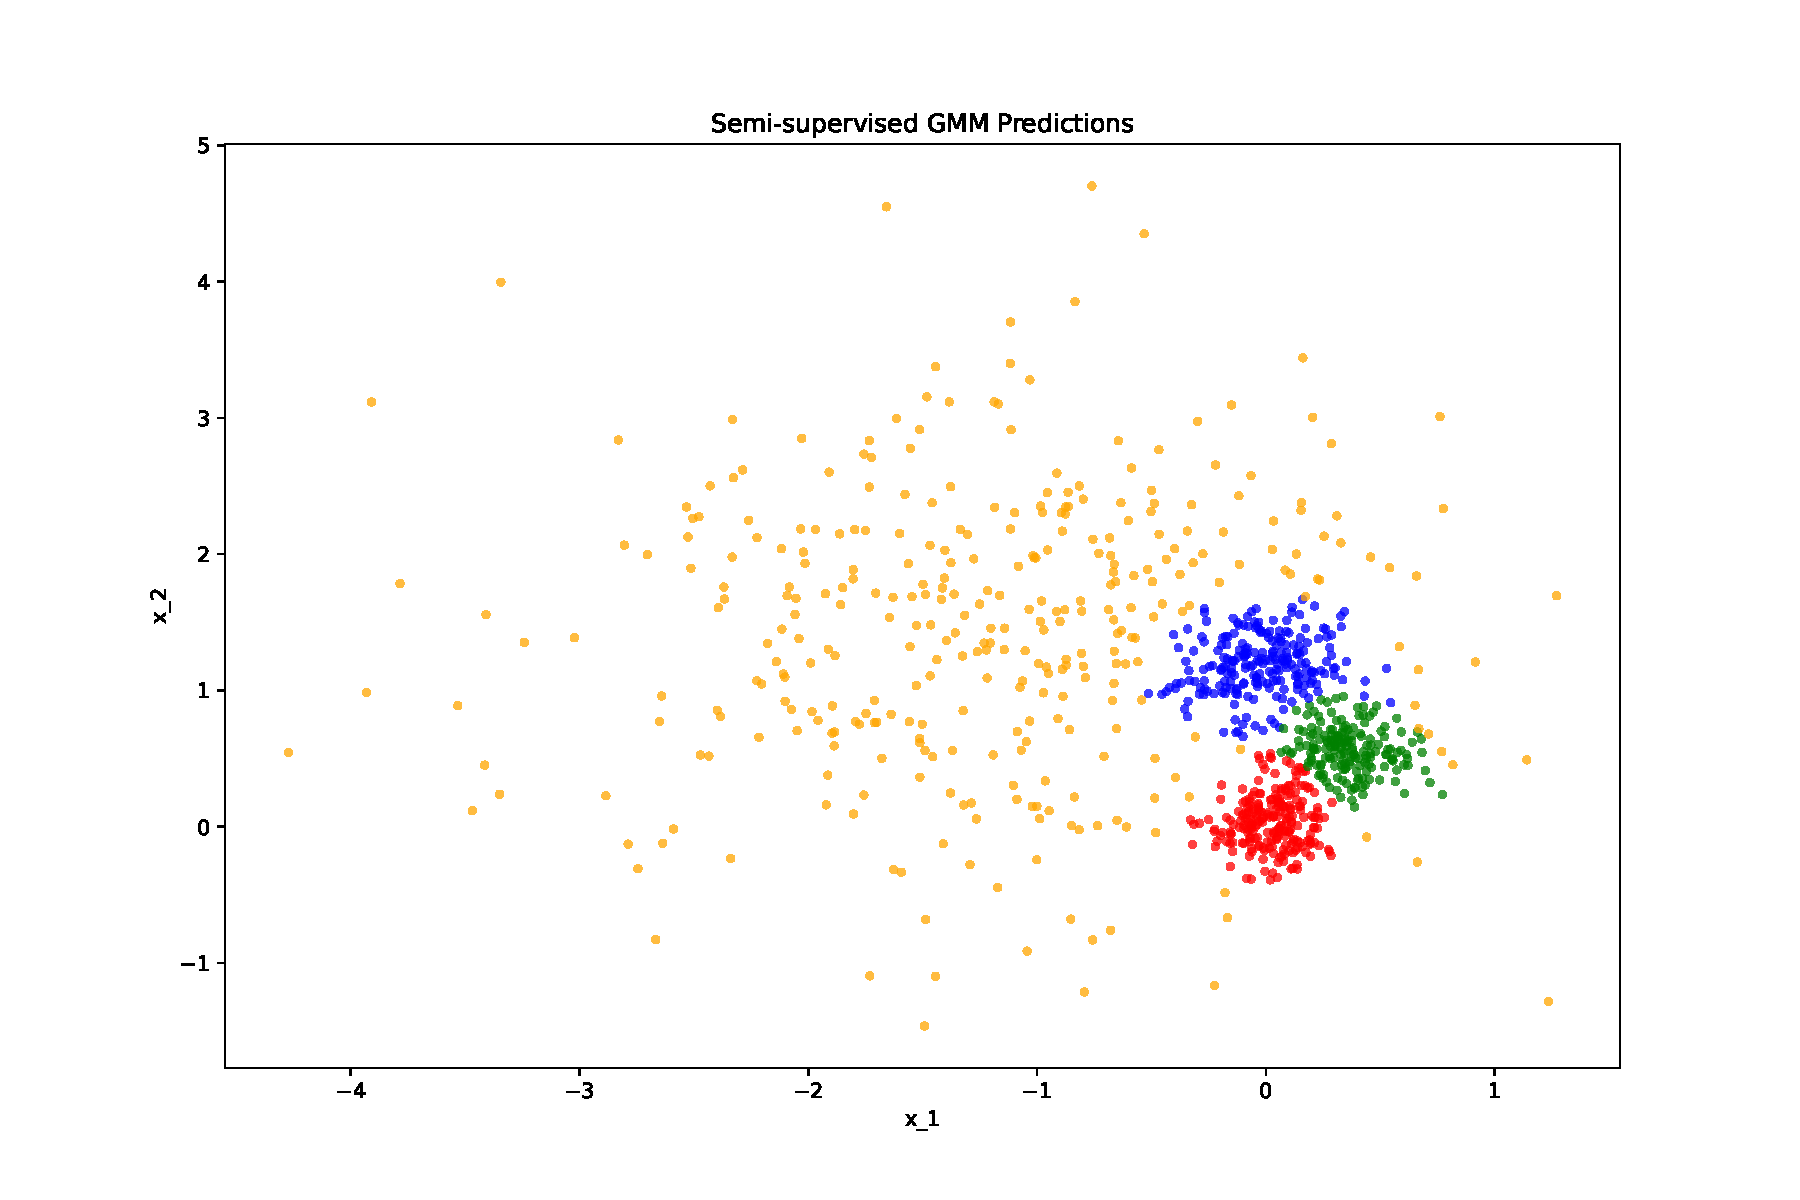
\includegraphics[width=1\textwidth]{images/p03_pred_ss_2.pdf}
  \caption{Semi-supervised GMM}
  \label{fig:enter-label}
\end{figure}

\newpage

\section*{Exercise 5}
\subsection*{(a),(b)}
After the compression, we represent each pixel with 4 bits(16 clusters), whereas in the original image each pixel took 24 bits, so the compression is by a factor of 6

\begin{figure}[h]
  \centering
  \includegraphics[width=1\textwidth]{images/image0.png}
  \caption{Small image}
  \label{fig:enter-label}
\end{figure}

\begin{figure}
  \centering
  \includegraphics[width=1\textwidth]{images/image1.png}
  \caption{Large image}
  \label{fig:enter-label}
\end{figure}

\begin{figure}
  \centering
  \includegraphics[width=1\textwidth]{images/image2.png}
  \caption{Large image after using K-means}
  \label{fig:enter-label}
\end{figure}


\end{document}

